% "Лаба"

\documentclass[a5paper,10pt, twoside]{article} % тип документа

\usepackage{import}


%  Русский язык

\import{../../headers/}{russian.tex}

% Математика

\import{../../headers/}{math.tex}

% Дефайны

\import{../../headers/}{my_defs.tex}


\graphicspath{{pics/}} % где лежат картинки

% Title Page
\title
{
\hfill \break	\hfill \break
\hfill \break	\hfill \break
Лабораторная работа 4.3.4.

ПРЕОБРАЗОВАНИЕ ФУРЬЕ В ОПТИКЕ
}
\author{Хайдари Фарид, Б01-901}


\begin{document}

\maketitle


\thispagestyle{empty} % выключаем отображение номера для этой страницы

\newpage

\tableofcontents % Вывод содержания

\newpage


\paragraph{Цель работы:}

исследование особенностей применения пространственного преобразования Фурье
для анализа дифракционных явлений.


\paragraph{В работе используются:}

гелий-неоновый лазер, кассета с набором
сеток разного периода, щель с микрометрическим винтом, линзы,
экран, линейка.

\section{Теоретические сведения}

Анализ сложного волнового поля во многих случаях целесообразно проводить, разлагая его на 
простейшие составляющие, например,представляя его в виде разложения по плоским волнам. При этом 
оказывается, что если мы рассматриваем поле, полученное после прохождения плоской 
монохроматической волны через предмет или транспарант (изображение предмета на фотоплёнке или 
стеклянной пластинке) с функцией пропускания t(x), то разложение по плоским волнам соответствует 
преобразованию Фурье от этой функции. Если за предметом поставить линзу, то каждая плоская волна 
сфокусируется в свою точку в задней фокальной плоскости линзы. Таким образом, картина, наблюдаемая 
в фокальной плоскости линзы, даёт нам представление о спектре плоских волн падающего на линзу 
волнового поля. Поэтому можно утверждать, что с помощью линзы в оптике осуществляется 
пространственное преобразование Фурье.

\subsection{Спектр функции пропускания амплитудной синусоидальной решётки}
	
	Рассмотрим вначале простой пример: дифракцию плоской монохроматической волны на синусоидальной
	амплитудной решётке. Пусть решётка с периодом $d$ расположена в плоскости $Z = 0$, а её штрихи 
	ориентированы вдоль оси $Y$ . Функция пропускания такой решётки имеет вид
	\begin{equation}\label{t_x}
		t(x) = \beta + \alpha \cos (ux) = \beta + \alpha \frac{\e^{iux} + \e^{-iux}}{2}
	\end{equation}
	с постоянными $\alpha$, $\beta$ и $u$ ($u = 2 \pi / d$ - пространственная частота) 
	
	Если на решётку падает плоская монохроматическая волна, распространяющаяся вдоль оси $Z$,
	\begin{equation}
		E(\vec{r}, t) = E_0 \e^{-i(\omega t - kz)}
	\end{equation}
	где $\omega$ -- круговая частота, $k$ -- волновой вектор ($k = 2\pi / \lambda$), $E_0$ -- 
	амплитуда, то на выходе из решётки мы получим три плоских волны:
	
	\begin{equation}\label{3E}
	\gath{
		E_1 = \beta \cdot E_0 \e^{-i(\omega t - kz)}; \\
		E_2 = \frac{\alpha}{2} \cdot \e^{-i(\omega t - ux - z \sqrt{k^2-u^2})}; \\
		E_3 = \frac{\alpha}{2} \cdot \e^{-i(\omega t + ux - z \sqrt{k^2-u^2})}.
	}
	\end{equation}
	
	Действительно, легко видеть, что в плоскости $Z = 0$ амплитуда колебаний, создаваемая суммой 
	этих волн, описывается функцией \eqref{t_x}, а фаза колебаний постоянна. Таким образом, в силу 
	единственности решения волнового уравнения при заданных граничных условиях мы нашли искомую 
	суперпозицию плоских волн. Каждая из этих трёх плоских волн фокусируется линзой в точку в 
	задней фокальной плоскости.
	
	Волна $E_1 = \beta \cdot E_0 \e^{-i(\omega t - kz)}$, распространяющаяся вдоль оси линзы 
	(оси $Z$), фокусируется в начало координат, а волны $E_2$ и $E_3$, распространяющиеся в 
	направлении $\sin{\theta} = \pm (u/k)$, фокусируются в точках 
	$x_{1-2} = \pm F u / k = \pm F \lambda / d$ ($F$ -- фокусное расстояние линзы).
	
	
	Функция $t(x)$ с самого начала задана в виде суммы гармонических составляющих, т.е. в виде 
	ряда Фурье. Каждой гармонической составляющей мы поставили в соответствие с \eqref{3E} 
	плоскую волну, собираемую линзой в точку в задней фокальной плоскости (её обычно называют 
	фурье-плоскостью). Проводя аналогию с «временной» координатой, мы можем заключить, что спектр 
	функции $t(x)$ представлен в фурье-плоскости тремя пространственными частотами: 0, $+u$, $-u$; 
	с амплитудами соответственно: $\beta, \alpha / 2, \alpha / 2$.
	
	Теорема Фурье, доказываемая в курсе математического анализа, утверждает, что широкий класс 
	периодических функций $t(x)$ может быть представлен в виде суммы бесконечного множества 
	гармонических составляющих, имеющих кратные частоты, т. е. в виде ряда Фурье. В комплексной 
	форме этот ряд имеет вид
	
	\begin{equation}\label{sum}
		t(x) = \sum_{n = -\infty}^{\infty} c_n \e^{i n u x}
	\end{equation}
	
	Рассуждая так же, как в случае амплитудной синусоидальной решётки, мы придём к выводу, что 
	картина, наблюдаемая в фурье-плоскости, представляет собой эквидистантный набор точек с 
	координатами
	
	\begin{displaymath}
		x_n = \frac{F u}{k} n = \frac{F \lambda}{d} n
	\end{displaymath}
	и амплитудами, пропорциональными $c_n$. Таким образом, с помощью линзы в оптике осуществляется
	пространственное преобразование Фурье: при освещении транспаранта плоской монохроматической 
	волной картина, наблюдаемая в задней фокальной плоскости линзы, установленной за 
	транспарантом, представляет собой фурье-образ функции пропускания транспаранта.
	
	Последнее утверждение нуждается в уточнении. Распределение света в задней фокальной плоскости 
	линзы будет воспроизводить распределение амплитуд плоских волн, продифрагировавших на 
	транспаранте, но фазовые соотношения при этом, вообще говоря, оказываются искажёнными и не 
	соответствуют аргументам комплексных амплитуд в выражении \eqref{sum}. При изменении 
	расстояния между транспарантом и линзой фазовые соотношения изменяются. Можно доказать, что 
	если транспарант установлен в передней фокальной плоскости линзы, то в её задней фокальной 
	плоскости восстанавливаются и амплитудные, и фазовые соотношения между плоскими волнами, и 
	таким образом строго осуществляется комплексное фурье-преобразование \eqref{sum}.
	
	Во многих практически важных случаях функция пропускания транспаранта чисто амплитудная, как,
		например, в случае амплитудной синусоидальной решётки \eqref{t_x}. Тогда для того, чтобы 
		найти фурье-образ функции пропускания транспаранта, достаточно определить только 
		пространственные частоты и соотношение между амплитудами плоских волн на выходе из 
		транспаранта. Для амплитудной синусоидальной решётки мы получили три плоских волны с 
		пространственными частотами 0, $+u, -u$ и амплитудами, пропорциональными 
		$\beta, \alpha / 2, \alpha / 2$. В соответствии с \eqref{t_x} мы можем утверждать, что 
		нашли пространственный фурье-образ функции пропускания амплитудной синусоидальной решётки.
	
	Интересно заметить, что наблюдаемая визуально картина фраунгоферовой дифракции в задней 
	фокальной плоскости линзы не зависит от расстояния между транспарантом и линзой, так как 
	глаз не реагирует на фазу волны, а регистрирует только интенсивность (усреднённый по времени 
	квадрат амплитуды поля). Условия наблюдения дифракции Фраунгофера можно выполнить и без 
	применения линзы, если наблюдать дифракционную картину на достаточно удалённом экране. 
	Таким образом, пространственное преобразование Фурье может осуществляться и в свободном 
	пространстве при наблюдении дифракции Фраунгофера.
	
\subsection{Спектр функции пропускания щелевой диафрагмы и периодической последовательности таких функций}
	
	Картина дифракции Фраунгофера на щели и на дифракционной решётке, имеющей вид периодического 
	набора щелей, хорошо известна из курса оптики. Спектр дифракционной решётки представлен на 
	рис. \ref{ris:dr}. Если размеры дифракционной решётки неограничены, то дифракционные 
	максимумы в спектре бесконечно узки. Чем меньше размер решётки	(полное число щелей), 
	тем шире каждый отдельный максимум.
	
	\begin{figure}[h]
		\begin{minipage}[h]{0.49\linewidth}
			\center{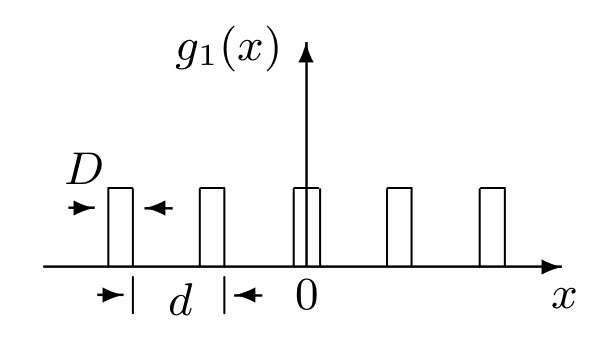
\includegraphics[width=0.7\linewidth]{1.png} \\ а)}
		\end{minipage}
		\hfill
		\begin{minipage}[h]{0.49\linewidth}
			\center{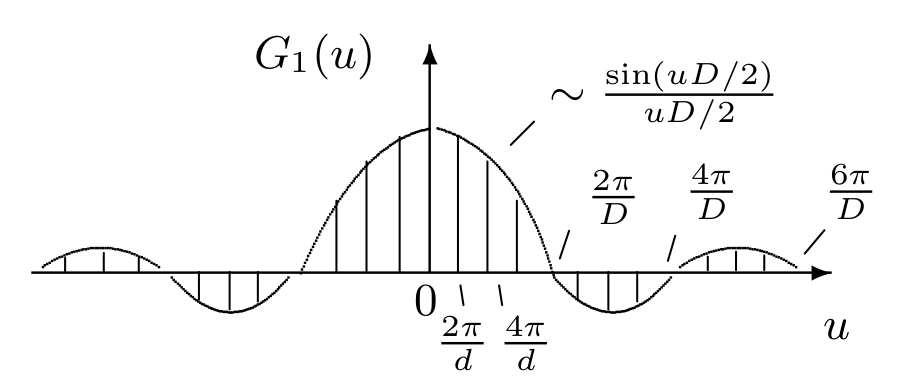
\includegraphics[width=1.1\linewidth]{2.png} \\ б)}
		\end{minipage}
		\caption
		{
			а) $g_1 (x)$ — функция пропускания дифракционной решётки (последовательности 
							прозрачных и непрозрачных полос); \\
			б) $G_1 (u)$ — спектр функции пропускания дифракционной решётки
		}
		\label{ris:dr}
	\end{figure}
	
	Направление на главные максимумы $\theta_n = un / k = \lambda n / d$ ($n$ -- целое число) 
	определяется периодом решётки $d$, а распределение амплитуд в спектре (огибающая) -- 
	фурье-образом функции пропускания отдельного штриха.
	
	\begin{equation}
		g_2(x) = 
		\system
		{
			1, -D / 2 \le x \le D / 2; \\ 
			0, -D / 2 > x > D / 2.
		}
	\end{equation}
	
	Так	как функция	$g_2(x)$ непериодична, её фурье-образ представляется непрерывным множеством 
	точек и определяется интегральным преобразованием Фурье:
	
	\begin{equation}
		\gath
		{
			g(x) = \frac{1}{2\pi} \Int_{-\infty}^{\infty} G(u) \e^{iux} du,\\
			G(u) = \Int_{-\infty}^{\infty} g(x) \e^{-iux} dx.
		}
	\end{equation}
	
	Говорят, что в таком виде $g(x)$ и $G(u)$ представляют собой пару преобразований Фурье: 
	$G(u)$ — спектр или фурье-образ функции $g(x)$.
	
	\begin{figure}[h]
		\begin{minipage}[h]{0.4\linewidth}
			\center{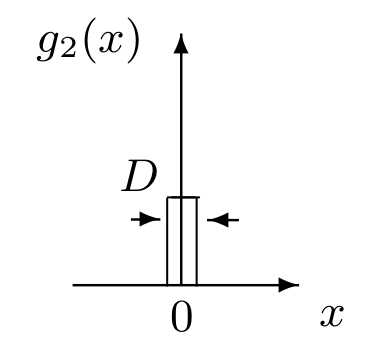
\includegraphics[width=0.7\linewidth]{3.png} \\ а)}
		\end{minipage}
		\hfill
		\begin{minipage}[h]{0.6\linewidth}
			\center{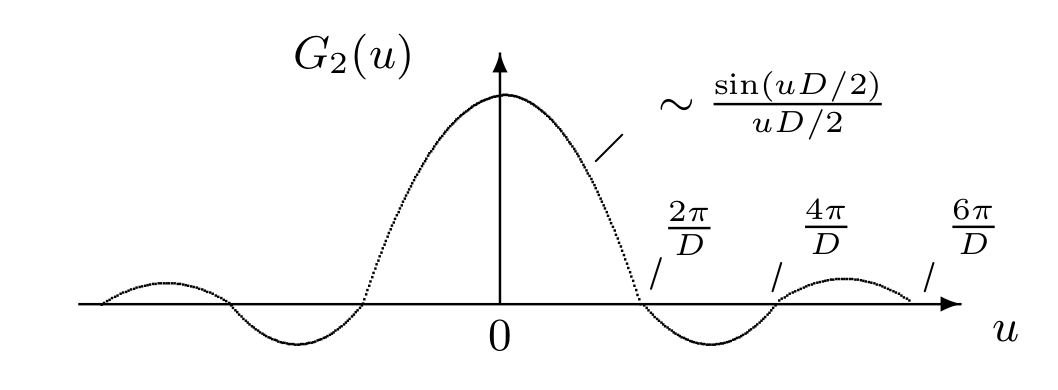
\includegraphics[width=1.1\linewidth]{4.png} \\ б)}
		\end{minipage}
		\caption
		{
			а) $g_1 (x)$ — функция пропускания щелевой диафрагмы; \\
			б) $G_1 (u)$ — спектр функции пропускания щелевой диафрагмы
		}
		\label{ris:dia}
	\end{figure}
	
	
	Спектр функции $g_2(x)$ хорошо известен, он соответствует картине дифракции Фраунгофера на 
	щели и описывается функцией вида $\frac{\sin x}{x}$ (рис. \ref{ris:dia}).
	
	Получим спектр $G_2(u)$ ещё раз с помощью преобразования Фурье:
	
	\begin{displaymath}
		G_2(u) = \Int_{-\infty}^{\infty} g_2(x) \e^{-iux} dx = \Int_{D / 2}^{D / 2} \e^{-iux} dx = D \frac{\sin (uD / 2)}{uD / 2}.
	\end{displaymath}
	
	Отсюда видно, что направление на первый минимум $\theta_1$ в огибающей спектра пропускания 
	дифракционной решётки определяется шириной функции пропускания отдельного штриха: 
	$\theta_1 = u / k = \lambda / D$. Если ввести понятия протяжённости функции пропускания 
	транспаранта по координате ($\Delta x$) и ширины её спектра ($\Delta u$), то
	
	\begin{equation}\label{ambiguity}
		\Delta u \cdot \Delta x = const.
	\end{equation}
	
	Для частного случая функции пропускания щелевой диафрагмы, определяя ширину её спектра по 
	первому нулю функции $\frac{\sin (uD / 2)}{uD / 2}$, получаем
	
	\begin{displaymath}
	\Delta u \cdot \Delta x = \frac{2 \pi}{D} \cdot D = 2 \pi.
	\end{displaymath}
	Соотношение \eqref{ambiguity} в волновой физике играет чрезвычайно важную роль. Его называют 
	соотношением неопределённости.
	
	Измерив на удалённом экране расстояния между максимумами или минимумами в спектре пропускания 
	щели (рис. \ref{ris:dia}б) или решётки (рис. \ref{ris:dr}б), можно рассчитать размер щели или 
	период решётки.
	
	Размер малого объекта можно рассчитать, если получить его изображение, увеличенное с помощью 
	линзы.
	
\subsection{Метод Аббе}
	
	Рассмотрим кратко схему образования изображения. Пусть предмет расположен в плоскости $P_1$ 
	на расстоянии от линзы большем, чем фокусное. Тогда существует сопряжённая предметной 
	плоскости $P_1$ плоскость $P_2$, где образуется изображение предмета-щели.
	
	\begin{figure}[h]
		\center{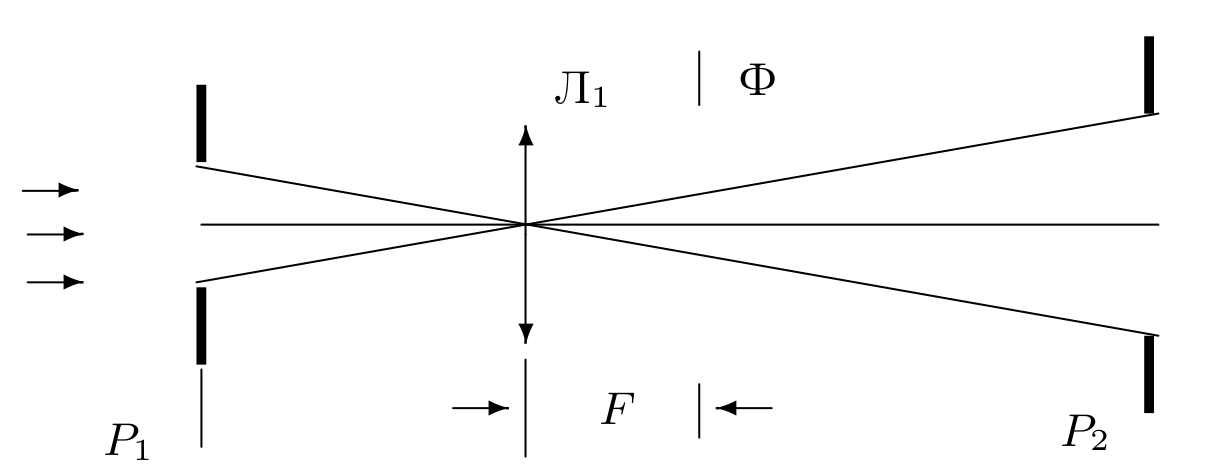
\includegraphics[width=1\linewidth]{5.png}}
		\caption{Схема, поясняющая метод Аббе построения изображения}
		\label{ris:abbe}
	\end{figure}
	
	Аббе предложил рассматривать схему прохождения лучей от предмета к изображению в два этапа. 
	Сначала рассматривается изображение спектр в задней фокальной плоскости Ф линзы $\text{Л}_1$ 
	(это изображение Аббе назвал первичным).
	
	Затем это изображение рассматривается как источник волн, создающий изображение предмет а в 
	плоскости $P_2$ (вторичное изображение). Такой подход опирается на принцип Гюйгенса–Френеля, 
	согласно которому любой участок волнового фронта можно рассматривать как источник излучения.
	
	\begin{figure}[h]
		\begin{minipage}[h]{0.65\linewidth}
			\center{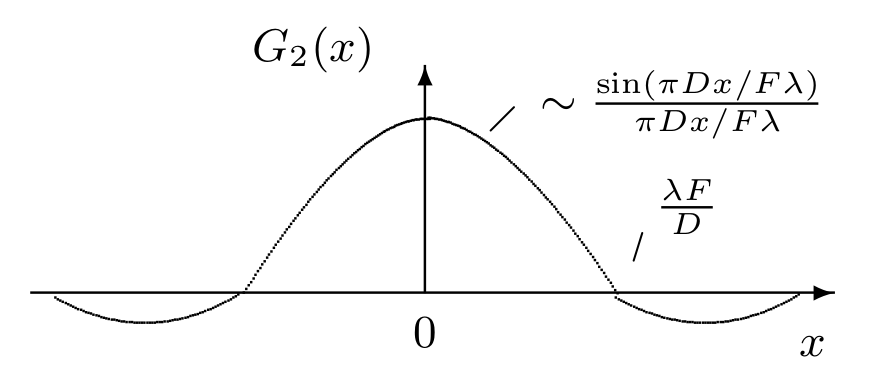
\includegraphics[width=1.0\linewidth]{6.png} \\ а)}
		\end{minipage}
		\vfill
		\begin{minipage}[h]{0.65\linewidth}
			\center{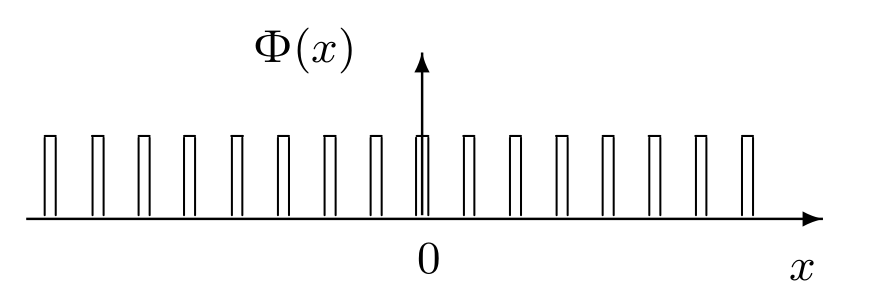
\includegraphics[width=1.0\linewidth]{7.png} \\ б)}
		\end{minipage}
		\vfill
		\begin{minipage}[h]{0.65\linewidth}
			\center{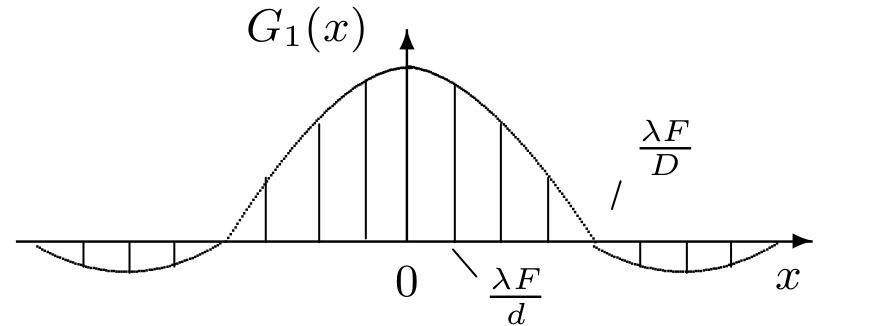
\includegraphics[width=1.0\linewidth]{8.png} \\ б)}
		\end{minipage}
		\caption
		{
			а) $G_2 (x)$ -- спектр функции пропускания щелевой диафрагмы; x -- координаты в 
							задней фокальной плоскости линзы; \\
			б) $\Phi_1 (x)$ -- функция пропускания решетки, установленной в фурье-плоскости 
								линзы;\\
			в) $G_1 (x)$ -- отфильтрованный спектр щелевой диафрагмы (ср. с рис. \ref{ris:dr})
		}
		\label{ris:three}
	\end{figure}
	
	Картина, наблюдаемая в плоскости $P_2$, зависит от распределения амплитуды и фазы в плоскости
	Ф -- в первичном изображении. Если плоскость $P_2$ сопряжена с предметной плоскостью
	$P_1$, то фазовые соотношения в первичном изображении оказываются именно такими, что в 
	плоскости $P_2$ мы наблюдаем соответственно увеличенное или уменьшенное изображение предмета. 
	Поэтому иногда говорят, что линза дважды осуществляет преобразование Фурье: сначала в задней 
	фокальной плоскости Ф линзы получается световое
	поле, соответствующее фурье-образу функции пропускания предмета (с точностью до фазы),	а 
	затем на промежутке между фокальной плоскостью Ф и плоскостью изображений $P_2$ 
	осуществляется обратное преобразование Фурье, и в плоскости $P_2$ восстанавливается таким 
	образом	изображение предмета.
	
	
\subsection{Мультипликация изображения предмета}

	Рассмотрим, что произойдёт с изображением предмета, если мы	установим в задней фокальной 
	плоскости линзы решётку. Сопоставим вначале спектры щелевой диафрагмы (рис. \ref{ris:dia}) и 
	периодической последовательности щелевых диафрагм (рис. \ref{ris:dr}).
	
	Легко видеть, что спектр, изображённый на рис. \ref{ris:dr}, можно получить из спектра, 
	изображённого на рис. \ref{ris:dia}, если исключить из него часть пространственных частот, 
	поместив в фурье-плоскость решётку -- последовательность прозрачных и непрозрачных линий 
	(рис. \ref{ris:three}).
	
	Отфильтрованный таким образом спектр не будет отличаться ни по амплитуде, ни по фазе от 
	спектра периодической последовательности щелевых диафрагм, и в плоскости $P_2$ мы получим 
	вместо изображения одиночной щели изображение периодической последовательности щелей.
	
	Эти рассуждения можно повторить и для предмета с произвольным спектром, необходимо только, 
	чтобы период решётки был заметно меньше ширины спектра (точное соотношение можно получить из 
	теоремы Котельникова). Таким образом, установив в задней фокальной плоскости линзы решётку, 
	мы вместо изображения одиночного предмет а получим эквидистантный набор изображений таких 
	предметов, т. е. осуществим мультипликацию изображения предмета (увидим изображение	
	несуществующей «фиктивной» решётки).
	
	Поменяв местами сетку и щель, можно проследить влияние размера щели на изображение сетки.
	
\section{Экспериментальная установка}

Схема установки представлена на рис. \ref{ris:ust}. Щель переменной ширины $D$, снабжённая 
микрометрическим винтом В, освещается параллельным пучком света, излучаемым
лазером (радиус кривизны фронта волны велик по сравнению с фокусными расстояниями используемых 
в схеме линз).

\begin{figure}[h]
	\center{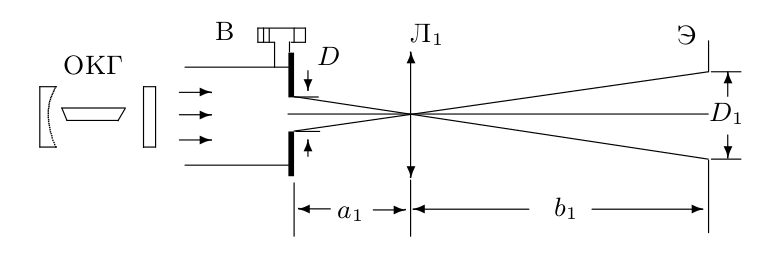
\includegraphics[width=1\linewidth]{9.png}}
	\caption{Схема для определения ширины щели с помощью линзы}
	\label{ris:ust}
\end{figure}

Увеличенное изображение щели с помощью линзы $\text{Л}_1$ проецируется на экран Э. Величина
изображения $D_1$ зависит от расстояний от линзы до предмета -- $a_1$ и до изображения -- $b_1$, 
т. е. от увеличения Г системы:

\begin{equation}
	\Gamma = \frac{D_1}{D} = \frac{b_1}{a_1}
\end{equation}\label{eq::zoom}

Изображение спектра щели образуется в задней фокальной плоскости Ф линзы $\text{Л}_1$. Размещая в 
плоскости Ф двумерные решётки-сетки, можно влиять на первичное изображение и получать 
мультиплицированное изображение щели.

\begin{figure}[h]
	\center{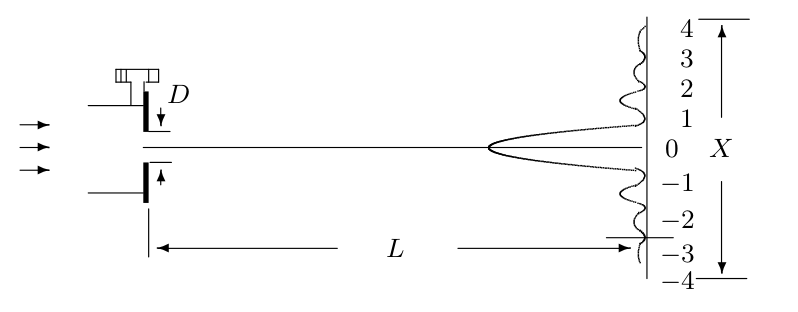
\includegraphics[width=1\linewidth]{10.png}}
	\caption{Схема для определения ширины щели по спектру}
	\label{ris:spectrum}
\end{figure}

\begin{figure}[h]
	\center{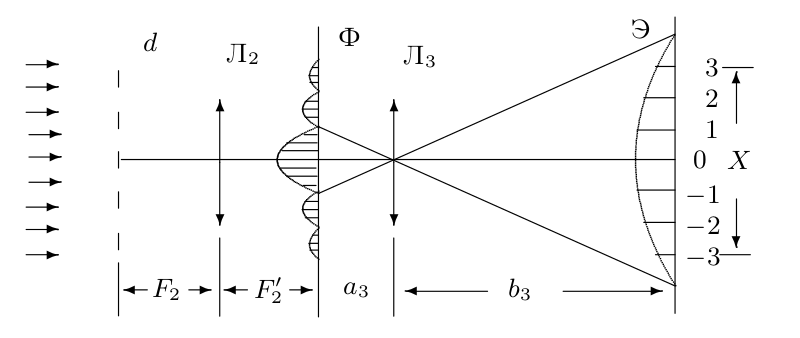
\includegraphics[width=1\linewidth]{11.png}}
	\caption{Схема определения периода решётки по увеличенному изображению спектра}
	\label{ris:d_per}
\end{figure}

Убрав линзу, можно наблюдать на экране спектр щели (рис. \ref{ris:spectrum}), а если заменить 
щель решёткой -- спектр решётки. Крупные решётки дают на экране очень мелкую картину спектра, 
которую трудно промерить. В этом случае используют две линзы (рис. \ref{ris:d_per}): первая 
(длиннофокусная) формирует первичное изображение -- спектр, вторая (короткофокусная) -- 
проецирует на экран увеличенное изображение спектра.




\section{Ход работы}

\subsection{Определение ширины щели}

\subsubsection{Определение ширины щели с помощью линзы}

	Схема установки изображена на рис. \ref{ris:ust}

	Измеряем расстояния $a_1$ и $b_1$ для определения увеличения $\Gamma$ системы: 
	$ a_1 = 4.5 \text{ см, } b_1 = 126.6 \text{ см} $. Находим те же $a_1$ и $b_1$ с помощью формулы 
	тонкой линзы: 
	$ a_1^{\text{теор}} \approx 3.9 \text{ см, } b_1^{\text{теор}} \approx 128.1 \text{ см} $.

	С помощью короткофокусной линзы $\text{Л}_1$ ($F_1 = 3.8$ см) получаем на экране $\text{Э}$
	увеличенное изображение щели. Меняя ширину щели от 50 до 500 мкм (5 - 50 делений от нового нуля), 
	снимаем зависимость размера изображения $D_1$ от ширины щели $D$. Также, зная величение линзы и
	размер изображения, рассчитаем по формуле \eqref{eq::zoom} ширину входной щели $D_{\text{Л}}$.

	% возможно нужно указать погрешности D и D_1
	\begin{table}[h]
		\center{\import{./src/}{dl.tex}}
		\caption{Зависимость размера изображения от ширины щели}
	\end{table}

\subsubsection{Определение ширины щели по её спектру}

	Получаем на удалённом экране спектр щели, как на рис. \ref{ris:spectrum}. Измеряем ширину спектра 
	для самой маленькой щели. Проводим серию измерений $X(m)$, меняя ширину щели в тех же
	пределах, что и в предыдущем пункте. Также измеряем расстояние $L$ от щели до экрана.

	По результатам измерений спектра рассчитываем ширину щели $D_c$ (<<c>> -- по спектру), используя
	соотношение

	\begin{equation}
		\Delta X = \frac{X}{2m} = \frac{\lambda}{D_c} L
	\end{equation}

	Длина волны He-Ne лазера $\lambda = 6328$ \AA.


	% почему-то не импортится
	\begin{table}[h]
		\begin{center}
			\begin{tabular}{| c | c | c | c | c | c | c |}
			\hline
			$D$, мкм & $m$ & $X$, мм & $\sigma_X$ & $D_c$, мм & мкм & $\sigma_{D_c}$\\
			\hline
			$10$ & $1$ & $142$ & $1$ & $0,01176$ & $11,76$ & $0,00008$\\
			\hline
			$10$ & $2$ & $286$ & $1$ & $0,01168$ & $11,68$ & $0,00004$\\
			\hline
			$60$ & $1$ & $28$ & $1$ & $0,060$ & $59,66$ & $0,002$\\
			\hline
			$60$ & $2$ & $54$ & $1$ & $0,0619$ & $61,87$ & $0,0011$\\
			\hline
			$100$ & $1$ & $17$ & $1$ & $0,098$ & $98,27$ & $0,006$\\
			\hline
			$100$ & $2$ & $33$ & $1$ & $0,101$ & $101,25$ & $0,003$\\
			\hline
			$200$ & $1$ & $8$ & $1$ & $0,209$ & $208,82$ & $0,03$\\
			\hline
			$200$ & $2$ & $17$ & $1$ & $0,197$ & $196,54$ & $0,012$\\
			\hline
			$200$ & $3$ & $25$ & $1$ & $0,200$ & $200,47$ & $0,008$\\
			\hline
			$300$ & $1$ & $6$ & $1$ & $0,28$ & $278,43$ & $0,05$\\
			\hline
			$300$ & $2$ & $11$ & $1$ & $0,30$ & $303,74$ & $0,03$\\
			\hline
			$400$ & $1$ & $4$ & $1$ & $0,42$ & $417,65$ & $0,10$\\
			\hline
			$400$ & $2$ & $9$ & $1$ & $0,37$ & $371,24$ & $0,04$\\
			\hline
			$580$ & $1$ & $3$ & $1$ & $0,56$ & $556,86$ & $0,19$\\
			\hline
			$580$ & $2$ & $6$ & $1$ & $0,56$ & $556,86$ & $0,09$\\
			\hline
			\end{tabular}
		\end{center}
		\caption{Зависимость размера изображения от ширины щели}
	\end{table}

	Строим графики $D_{\text{л}} = f(D)$ и $D_c = f(D)$.

	% график

	Таким же образом определяем ширину волоса

	% волос

\subsection{Определение периода решёток}

	\subsubsection{Определение периода по спектру на удалённом экране}

	\subsubsection{Определение периода решёток по увеличенному изображению спектра}

\subsection{Мультиплицирование}

	

\end{document} % конец документа
